% https://es.overleaf.com/latex/templates/project-report/jpzczmpsdzwm

%%% Preamble
\documentclass[paper=leter, fontsize=11pt]{scrartcl}
\usepackage[utf8]{inputenc}
\usepackage[spanish,mexico]{babel}
\usepackage[T1]{fontenc}    % use 8-bit T1 fonts
\usepackage{lmodern}
\usepackage{hyperref}       % hyperlinks
\usepackage{lipsum}
\usepackage[square,numbers]{natbib}

\usepackage[protrusion=true,expansion=true]{microtype}	
\usepackage{amsmath,amsfonts,amsthm} % Math packages
\usepackage[pdftex]{graphicx}
\usepackage{url}

\usepackage{booktabs}

\usepackage{tikz}
\usetikzlibrary{positioning,matrix, arrows.meta}

\usepackage{caption}
\usepackage{subcaption}

\usepackage{listings}
\lstdefinestyle{mystyle}{
    basicstyle=\ttfamily\footnotesize,
    breakatwhitespace=false,         
    breaklines=true,                 
    captionpos=b,                    
    keepspaces=true,                 
    numbers=left,                    
    numbersep=5pt,                  
    showspaces=false,                
    showstringspaces=false,
    showtabs=false,                  
    tabsize=4
}

\lstset{style=mystyle}
\renewcommand{\lstlistingname}{Código}

\graphicspath{ {img/} }

\selectlanguage{spanish}
\usepackage[spanish,onelanguage,ruled]{algorithm2e}


%%% Custom sectioning
\usepackage{sectsty}
\allsectionsfont{\centering \normalfont\scshape}


%%% Custom headers/footers (fancyhdr package)
\usepackage{fancyhdr}
\pagestyle{fancyplain}
\fancyhead{}											% No page header
\fancyfoot[L]{}											% Empty 
\fancyfoot[C]{}											% Empty
\fancyfoot[R]{\thepage}									% Pagenumbering
\renewcommand{\headrulewidth}{0pt}			% Remove header underlines
\renewcommand{\footrulewidth}{0pt}				% Remove footer underlines
\setlength{\headheight}{13.6pt}


%%% Equation and float numbering
\numberwithin{equation}{section}		% Equationnumbering: section.eq#
\numberwithin{figure}{section}			% Figurenumbering: section.fig#
\numberwithin{table}{section}				% Tablenumbering: section.tab#


%%% Maketitle metadata
\newcommand{\horrule}[1]{\rule{\linewidth}{#1}} 	% Horizontal rule

%%% https://tex.stackexchange.com/a/118217
\usepackage{mathtools}
\DeclarePairedDelimiter\ceil{\lceil}{\rceil}
\DeclarePairedDelimiter\floor{\lfloor}{\rfloor}

\usepackage{amsmath}

\usepackage{tikz}

\title{
		%\vspace{-1in} 	
		\usefont{OT1}{bch}{b}{n}
		\normalfont \normalsize \textsc{Posgrado de Ingeniería de Sistemas} \\ [25pt]
		\horrule{0.5pt} \\[0.4cm]
		\huge Algoritmo de aproximación al problema de la mochila \\
		\horrule{2pt} \\[0.5cm]
}
\author{
		\normalfont 								\normalsize
        Alberto Benavides\\[-3pt]		\normalsize
        \today
}
\date{}


%%% Begin document
\begin{document}
\maketitle

\section{Problema de la mochila}
El \textit{problema de la mochila} consiste en tener un contenedor de capacidad definida y un conjunto $C$ de $n$ objetos de determinados peso $p$ y valor $v$, de los que se desea seleccionar el subconjunto con el mayor valor entre la suma de los valores de los objetos que lo componen, sin que la suma de sus pesos supere la capacidad del contenedor.

Para encontrar este subconjunto se exploran todos los subconjuntos hasta encontrar el que cumpla con las condiciones dadas. Esto implica revisar $2^n$ subconjuntos, lo que toma un tiempo $\mathcal{O}(2^n)$. Intuitivamente, se puede decir que en instancias grandes, se requiere un gran poder de procesamiento o mucha paciencia para obtener el resultado exacto.

En situaciones donde se requiere un resultado funcional en poco tiempo, se pueden utilizar metodologías alternativas para obtenerlo. En el caso del problema de la mochila, una estrategia es ordenar los objetos por la relación que hay entre su valor y peso $v / p$ e insertarlos en ese orden en el contenedor mientras no superen la capacidad ya citada. Esta opción toma un tiempo que depende del algoritmo usado para ordenar. Para esta práctica se realizó un diseño de experimentos que utiliza la función \texttt{sort} \cite{python-sort} de \texttt{Python}, la cual tiene una complejidad computacional $\mathcal{O}(n \log{n})$ \cite{python-sort-complexity}.

\section{Diseño de experimentos}

Para conocer las diferencias entre el tiempo de ejecución y la distancia al mayor valor alcanzado del algoritmo exacto con respecto al aproximado, se ejecutan $10$ repeticiones de ambos algoritmos con tamaños de conjuntos $N = [2, 25]$ que tienen valores y pesos asignados al azar entre $[0, 1]$ desde una distribución normal. Esta experimentación se realiza en una computadora con Windows 10, procesador i7-9750H de $2.60$ GHz y $32$ GB de memoria RAM, en \texttt{Python v. 3.8}.

\section{Resultados}

Tras realizar los experimentos computacionales descritos en la sección anterior, se observa que los tiempos de ejecución del algoritmo aproximado son inferiores a $00.000997$ segundos, por lo que pueden considerarse despreciables. Por su parte, los del algoritmo exacto tienen crecimiento exponencia como se plasma en la figura \ref{tiempo_mejores}.

Ahora bien, para conocer el porcentaje de similitud del algoritmo aproximado con el exacto se dividió cada suma de valores obtenida por uno y otro algoritmo para la misma réplica, de donde se obtuvo una similitud del $100 \%$ o cercana con sólo $10$ réplicas de cada ejecución del algoritmo aproximado, lo cual puede revisarse en la figura \ref{porcentaje}.

\begin{figure}
    \centering
    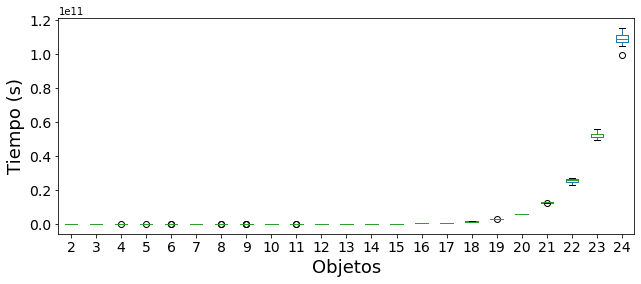
\includegraphics[width=0.8\textwidth]{tiempo_mejores.png}
    \caption{Tiempos de ejecución del algoritmo exacto en segundos, dado un número de objetos.}
    \label{tiempo_mejores}
\end{figure}

\begin{figure}
    \centering
    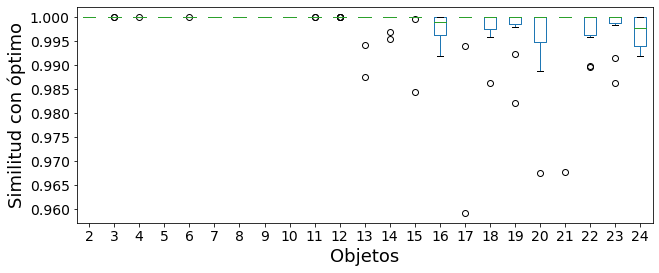
\includegraphics[width=0.8\textwidth]{porcentaje.png}
    \caption{Grado de similitud entre los valores óptimos y aproximados por número de objetos.}
    \label{porcentaje}
\end{figure}

Para revisar si el número de objetos afecta la similitud del valor aproximado al óptimo, se realiza un análisis estadístico. Primero, se prueba si hay homogeneidad de variables por la prueba de Levene, con lo que se obtiene un $p$-valor de $1.08\times10^{-98}$ que denota la ausencia de homogeneidad, por lo que se realiza una prueba de Welch entre las variables que da por $p$-valor $3.78\times10^{-74}$, o sea que se rechaza la nula hipótesis para aceptar que existe diferencia significativa entre el número de objetos y la similitud del valor apróximado frente al óptimo, lo que puede intuirse debido a que, a menor cantidad de objetos, es más probable que se incluyan los mismos por los distintos algoritmos.

\section{Comentarios finales}
Con estos resultados se puede concluir que en casos en que se pueda tener cierta holgura en la precisión de la obtención de valores cercanos al óptimo, es recomendable utilizar algoritmos de aproximación, en especial si se requieren resultados en cortos periodos de tiempo. Podría extenderse esta experimentación al realizarla con más objetos y conocer la manera en que afecta el tamaño de muestra a la similitud entre valores aproximado y óptimo.

Los algoritmos y experimentos aquí discutidos pueden encontrarse en \url{https://tinyurl.com/y878q6lk}. 

\bibliographystyle{plainnat}
\bibliography{Biblio}

\end{document}